\chapter{Svolgimento del Tirocinio}

In questo capitolo verrà spiegato nel dettaglio lo svolgimento del tirocinio. L'obiettivo preposto è stato quello di realizzare un'applicazione funzionante per visualizzare e gestire mappe geospaziali. Lo sviluppo si è diviso tra front-end, per consentire la visualizzazione delle mappe, e back-end, per la loro gestione e fornitura. Infine, si è concluso il mio percorso lavorativo con una fase di integrazione tra i due componenti.

\section{Sviluppo Front-end con OpenLayers}

\subsection{Perché OpenLayers}

Tale libreria è stata scelta, rispetto alle altre concorrenti, in quanto offre internamente molte funzionalità utili per la rappresentazione di questo tipo di mappe.
\\Come già spiegato nel secondo capitolo, OpenLayers offre un supporto già integrato ai protocolli OGC, essenziali per la rappresentazione di questi tipi di dati geospaziali. La maggior parte delle sorgenti di mappe fornite, infatti, sono trasmesse mediante protocolli OGC quali WMS, WFS e WCS. Con l'utilizzo di questa libreria, la comunicazione ai servizi OGC esterni risulta essere più semplice, in quanto non è necessario eseguire manualmente tutte le richieste imposte dallo Standard, e, successivamente, eseguire il parsing sul contenuto delle risposte in formato XML. OpenLayers fornisce, a più livelli, delle classi che si occupano di eseguire queste operazioni al posto nostro, e attraverso il principio di Information Hiding, espongono allo sviluppatore solo il minimo necessario per eseguire correttamente la richiesta.
\\Per esempio, nel caso dell'implentazione del protocollo WMS, non sarà quindi necessario eseguire una richiesta di GetCapabilities e successivamente GetMap, al fine di ricevere l'immagine della mappa. Se il nome del layer è noto, basterà istanziare la classe ImageWMS che passandogli i parametri corretti, eseguirà automaticamente le operazioni necessarie al fine di ricevere l'immagine della mappa corretta. Qui sotto viene riportato un esempio di implementazione della classe ImageWMS, il quale è possibile reperire anche dalla documentazione di OpenLayer\cite{DocumentazioneOpenLayersWMS}
\lstinputlisting[language=Java, caption={Esempio di ImageWMS}]{listings/Capitolo3/openLayerWMS.js}
Come si può vedere dall'esempio, al fine di recuperare l'immagine della mappa fornita dal server WMS esterno, è necessario istanziare la classe ImageWMS passandogli come argomento soltanto l'URL e il layer che si vuole visualizzare.
OpenLayer si occuperà di eseguire la richiesta di GetMap al posto nostro e di mostrare a schermo l'immagine della mappa.
\\Tale esempio richiede ovviamente che il nome del layer sia noto, nel caso in cui il client non conosca la lista di layer disponibili, sarà comunque necessario eseguire una richiesta di GetCapabilities.
\\Anche in questo caso, OpenLayer si occupa di eseguire la richiesta e di effettuare il parsing in automatico sul contentuo dell'XML, senza dover creare una struttura dati apposita per manipolare i dati ricevuti da essa.
\lstinputlisting[language=Java, caption={Esempio di GetCapabilities per WMS}]{listings/Capitolo3/openLayerWMSCapabilities.js}
Inoltre la libreria ha già un supporto integrato per il formato GeoJSON, il che la rende ottimale al fine di testare le mappe fornite da IdroGEO, in quanto quest'ultime non vengono distribuite mediante un servizio OGC, ma vengono fornite come file locali in formato GeoJSON.
\\Infine, la libreria è interamente supportata da Angular e con un semplice comando di npm (mpm install ol), la si può installare all'interno del progetto, il che la rende ottimale per questo tipo di applicazione.

% poi spiego come ho fatto l'applicazione
% poi spiego i problemi come li ho affrontati (pro4j, geojson)

\subsection{Implementazione nel Progetto}

Il candidato, sotto supervisione del tutor aziendale, ha iniziato lo sviluppo del progetto BMS creando all'interno dell'applicazione una nuova pagina web, nella quale ha importato il componente della mappa già esistente nell'Ui-Kit, così da poter integrare il supporto ai protocolli OGC richiesti e iniziare a testare le mappe censite.
\\Lo sviluppo è proseguito estenendo il componente Angular delle mappe, che fino a quel momento ha presentato solamente l'integrazione agli elementi base di OpenLayers e un supporto alla sovrapposizione multipla di layer differenti.
\\Come prima funzionalità si è implementato il supporto al formato GeoJSON, selezionando come prima mappa da testare quella delle frane in Toscana, fornita da IdroGEO, in quanto tutte quelle fornite da questo ente, possono essere scaricate localmente e caricate all'interno del progetto, senza dover contattare alcun servizio esterno. Ciò facilità il lavoro di programmazione, riducendo il rischio di errore dovuto a eventuali problemi di disservizio dei server di mappe esterni.
\\In questa fase, le parti di codice che hanno subito più modifiche sono le classi BuildLayer.ts e MapModel.ts, le quali si occupano di far istanziare l'oggetto della mappa con proprietà differenti, in base al tipo di formato geospaziale passato come argomento.
\\Il lavoro è continuato con l'implementazione della classe descritta precedentemente (pagina web), andando a inserire al suo interno alcune mappe fittizie, tra cui una in formato GeoJSON, così da poterne verificare il funzionamento. Tali mappe, rappresentate come "layer", sono state tutte sovrapposte a quella di default, ovvero la mappa di OpenStreetMap. In questo modo si è compreso se i layer sono stati rappresentati correttamente, riuscendo così a orientarsi all'interno delle mappe stesse in termini geografici.

voglio dire che ho aggiunto il layer di openstreet map
voglio dire del problema di pro4j
voglio dire del problema di clustering e la ram mangiata
voglio dire dello stile applicato e il click dei marker


\lstinputlisting[language=Java, caption={Implementazione BuildLayer}]{listings/Capitolo4/buildLayer.js}




% in questa fase il lavoro si è prevalentemente incentrato sulla classe BuildLayer.ts, la quale si occupa di bababababab. Alla seguente classe sono stato apportate le seguenti modifiche: basdbsamdasbdnas


% * oh no! non va na sega! usiamo pro4j *





% è stato scelta una mappa di IdroGEO in formato geojson, perché


% Abbiamo preso i link dei dati delle mappe che ho censito i primi giorni. Abbiamo scelto un link del sito blu (quello idrico) e abbiamo provato a prendere il file delle frane della toscana in formato GeoJson e darlo in pasto a open layer, nella speranza che in automatico riuscisse a capire quei dati e mostrarli a schermo.
% Abbiamo quindi creato un nuovo tipo e fornito nella condizione dello switch case iniziato da Alessandro (lui aveva fatto funzionare i tipi: assets, tiles, topojson, ma non geojson!)
% Abbiamo creato un nuovo layer con new GeoJson() supportato direttamente da open layer.
% Abbiamo definito lo stile in cui i dati nel file geojson dovevano essere rappresentati (dei cerchi rossi in svg).
% A quanto pare il formato geojson serve per disegnare roba nella mappa, come coordinate punti o linee, non mappe. Di conseguenza ci serve uno stile da dare a open layer con cui deve leggere.
% A questo punto abbiamo fatto renderizzare la mappa a schermo ma senza successo. Il codice era scritto correttamente ma il sistema di coordinate passato dal file geojson era sconosciuto a open layer.
% Quindi abbiamo creato una nuova projection con le chiamate fornite della libreria e abbiamo definito il funzionamento di quella projection con una libreria chiamata `proj4`.
% Questa libreria permette di fare in automatico il cambio di coordinate da un sistema di riferimento ad un altro. Quindi e’ bastato fare la conversione e dare il risultato ad open layer.
% Poiche’ il file era di 64 Mega, e la quantita’ di dati era cosi densa, la mappa e’ arrivata a consumare la bellezza di 27 GB di ram prima di andare poi in swap e crashare. Quindi e’ stato necessario ‘clasterizzare’ i dati. Fortunatamente anche qui, open layer ci da una mano con una funzione cluster

% proiezione con pro4j,




% \section{Questa è una sezione}

% \lipsum[2]

% \subsection{Questa è una aaaaaa}

% \lipsum[3]

% \subsubsection{Questa è una sotto-sottosezione}

% \lipsum[4]

% É possibile riferire l'immagine, una volta assegnatagli una label, tramite il comando \texttt{\textbackslash autoref\{fig:immagine\}}, ottenendo il seguente risultato: \autoref{fig:immagine}.

% \begin{figure}
%     \centering
%     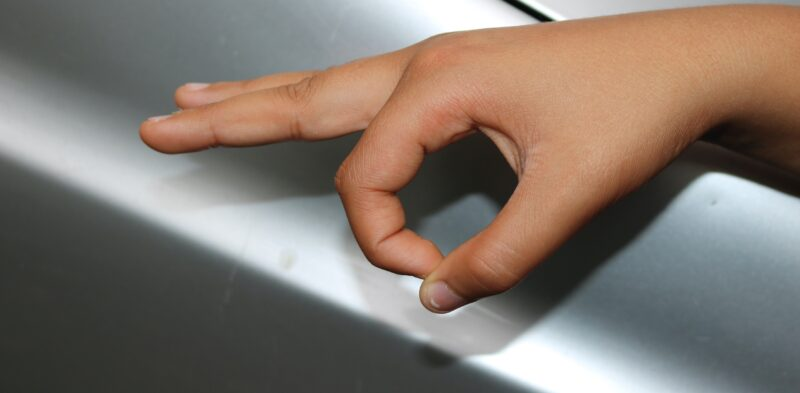
\includegraphics[width= 0.8\textwidth]{images/Capitolo1/immagine.jpg}
%     \caption{Questa è un'immagine}
%     \label{fig:immagine}
% \end{figure}

% Questa è una citazione \cite{LabelPerLaCitazione}.

% \subsubsection{Questa è un'altra sottosezionelipsum}

% Quello che segue è un esempio di codice. E' possibile modificare il linguaggio per il synyax highlight, aggiungere parole chiave... E' tutto disponibile nella guida del pacchetto \texttt{listings}.

% \lstinputlisting[language=C++]{listings/Capitolo1/code1.cpp}

% \section{Questa è un'ennesima sezione}

% \lipsum[4]

% \subsection{Sottosezione con una tabella}

% La tabella si indirizza sempre con l'uso di una label, ottenendo il risultato \autoref{tab:labelTabella}.

% \begin{table}
%     \caption{Una simpatica tabella!}\label{tab:labelTabella}
%     \begin{center}
%         \begin{tabular}{c|c|c|c}
%             \textbf{Colonna 1} & \textbf{Colonna 2} & \textbf{Colonna 3} & \textbf{Colonna 4} \\
%             \hline
%             $3$                & $24$               & $24$               & $29$               \\
%             $36$               & $31$               & $49$               & $39$               \\
%             $32$               & $41$               & $59$               & $57$               \\
%             $34$               & $60$               & $79$               & $74$               \\
%             $328$              & $96$               & $194$              & $99$               \\
%             $356$              & $117$              & $297$              & $149$              \\
%             $312$              & $315$              & $293$              & $242$              \\
%             $3024$             & $184$              & $253$              & $019$              \\
%             $3048$             & $7795$             & $253$              & $077$              \\
%             $3096$             & $7767$             & $2432$             & $0514$             \\
%             $3192$             & $3769$             & $2435$             & $0551$             \\
%             $36384$            & $6625$             & $3432$             & $0497$             \\
%             $32768$            & $15469$            & $6472$             & $0471$             \\
%             $35536$            & $15425$            & $14539$            & $10289$            \\
%             $331072$           & $34623$            & $24941$            & $20444$            \\
%         \end{tabular}
%     \end{center}
% \end{table}